\documentclass[conference]{IEEEtran}
\usepackage{graphicx,cite,bm,psfrag,amsmath}
\def\mmax{\mathop{\mbox{\scriptsize max}}}
\def\argmin{\mathop{\mbox{arg\,min}}}
\def\argmax{\mathop{\mbox{arg\,max}}}
\newcommand{\defequal}{\stackrel{\mathrm{def}}{=}}
\renewcommand{\vec}[1]{{\ensuremath{\boldsymbol{#1}}}}
\newcommand{\popt}{\ensuremath{P^{(K)}_{opt}}}
\IEEEoverridecommandlockouts
\pagestyle{plain}
\usepackage{amsfonts}
\usepackage{algorithm, algorithmic}
\renewcommand{\algorithmicrequire}{ \textbf{Input:}} %Use Input in the format of Algorithm
\renewcommand{\algorithmicensure}{ \textbf{Procedures:}} %UseOutput in the format of Algorithm
% correct bad hyphenation here
%\hyphenation{op-tical net-works semi-conduc-tor}
\usepackage{CJK}
\usepackage{color}
\usepackage{url}
\usepackage{geometry}
\geometry{left=0.5in, right=0.5in, top=0.75in, bottom=0.75in}

\begin{document}
\title{Group Scheduling for Block Diagonal Digital Precoder in Multi-user MIMO System}
\author{\IEEEauthorblockN{Guanchong Niu and Man-On Pun\IEEEauthorrefmark{3}
%\IEEEauthorrefmark{3},
\IEEEauthorblockA{
School of Science and Engineering\\
The Chinese University of Hong Kong, Shenzhen\\
Shenzhen, Guangdong, China, 518172
%\thanks{This work was supported, in part, by the CUHKSZ President's Fund under Grant No. PF.01.000211 and  Shenzhen Science and Technology Innovation Committee under Grant No. ZDSYS20170725140921348.} \thanks{\IEEEauthorrefmark{3} Corresponding author, email: SimonPun@cuhk.edu.cn.}
}}}


\maketitle \thispagestyle{plain}
\pagenumbering{gobble}

\begin{abstract}
Beam division multiple access (BDMA) has recently been proposed for massive multiple-input multiple-output (MIMO) systems by simultaneously transmitting multiple users' data streams via different beams. In our previous work, single-path propagation channel model has been investigated by opportunistically selecting users to suppress the multiuser interference. Similarly, for multipath channel model, the different paths of each user can be chosen opportunistically. Furthermore, the block diagonal precoding is proposed and the number of RF chains can be significantly reduced by applying the Time Division Duplex(TDD) or switches. Simulation results confirm the effectiveness of proposed block diagonal precoding algorithm.
\end{abstract}

\section{introduction}
To meet the ever-increasing demand of higher user data rates, it is envisioned that the next-generation cellular systems will be equipped with massive antenna arrays \cite{boccardi2014five}. Capitalizing on the large number of antennas at the base-station (BS), beam division multiple access (BDMA) has recently been proposed to transmit multiple users' data streams via different beams \cite{sun2015beam, Jiang2018}. In contrast to the more conventional multiple access schemes such as Code Division Multiple Access (CDMA) or Orthogonal Frequency Multiple Division Access (OFDMA) that multiplex users in code, time and frequency domains, BDMA separates users in the beam space by transmitting data to different users in orthogonal beam directions. In \cite{sun2015beam}, BDMA was first proposed to decompose the multiuser multiple-input multiple-output (MU-MIMO) system into multiple single-user MIMO channels by multiplexing multiple users' data onto non-overlapping beams. More recently, joint user scheduling and beam selection for BDMA was formulated under the Lyapunov-drift optimization framework before the optimal user-beam scheduling policy was derived in a closed form \cite{Jiang2018}.

In the meantime, hyrbid digital and analog beamforming has also been developed for millimeter wave (mmWave) massive MIMO transmissions by dividing the procoding process into two steps, namely analog and digital precoding \cite{han2015large, el2014spatially}. More specifically, the transmitted signals are first precoded digitally using a smaller number of radio frequency (RF) chains followed by the analog precoding implemented with a much larger number of low-cost phase shifters. As a result, the hybrid analog-digital precoding architecture requires significantly less RF chains as compared to the fully digital precoding in which every available antenna element is supported by one RF chain. 

\begin{figure}[h]
	\begin{center}
		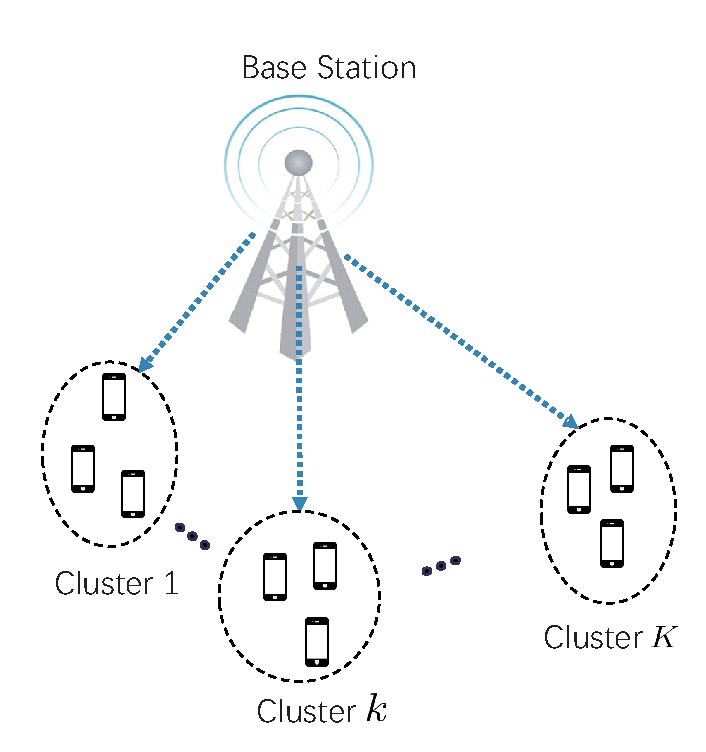
\includegraphics[scale=0.55]{PPTFigure/groupcluster.eps}
		\caption{Group scheduling to reduce the number of RF chains and eliminate the intra-cluster interference}\label{fig:BDMA}
	\end{center}
\end{figure}

{\color{red}However, the number of RF chains is lower bounded by the transmitted the number of data streams. In our proposed system, the users are grouped to several clusters. We assume the symbol duration is much larger than time delay thus the received symbols of different users are same and the channel gain is constant. Compared to serve each cluster separately, the interference will increase since each user has to decode received signal from other clusters. Leveraging the scheduling of users, we can firstly use analog precoding to eliminate the inter-cluster interference between cluster and then implement digital precoding to suppress the intra-cluster interference. The simulation results show that our proposed algorithm can efficiently reduce the number of RF chains without introducing large intra-cluster interference.} 

\underline{Notation}: Vectors and matrices are denoted by boldface letters. ${\bm A}^T$ and ${\bm A}^H$ denote transpose and conjugate transpose of ${\bm A}$, respectively. $\bm{A}^\dagger$ being the pseudo inverse of $\bm{A}$ while $||\bm{A}|| $ and $|\bm{A}|$ stand for the Frobenius norm and determinant of ${\bm A}$, respectively. $\bm{A}(i,j)$ denotes the $i$ row, $j$ column element of ${\bm A}$; $|\mathcal{I}|$ is the cardinality of the enclosed set ${\cal I}$; Finally, $\mathbb{E}[\cdot] $ and $\Re\{\cdot\}$ denote the expectation and real part of a random variable.

\begin{figure*}[htpb]
	\centering
	\begin{minipage}[t]{0.7\linewidth}
		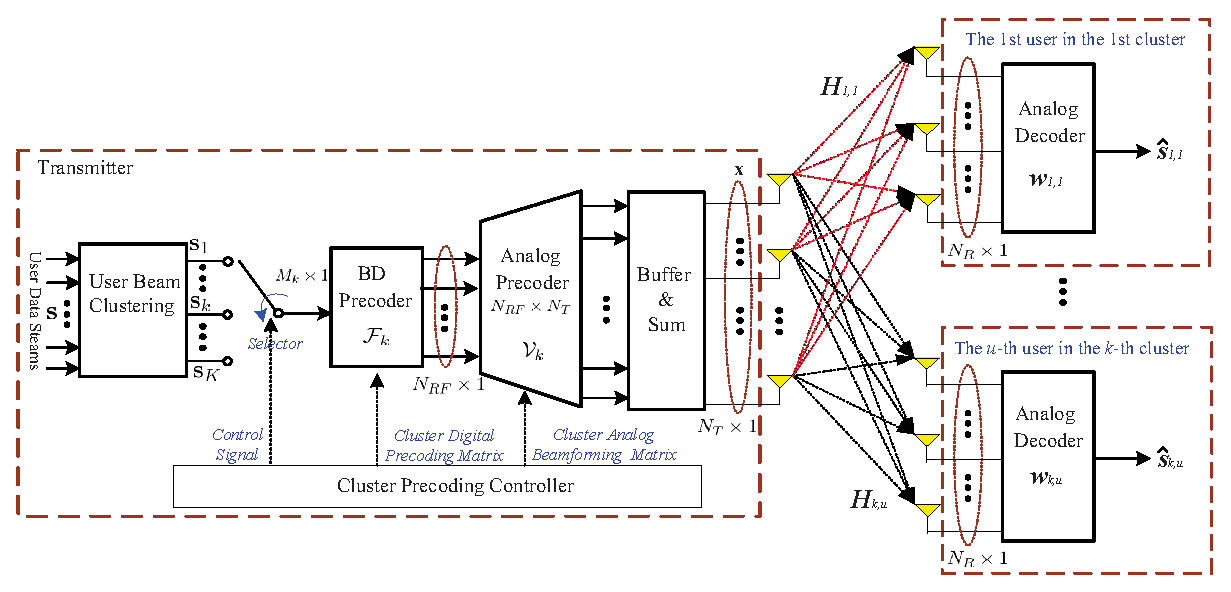
\includegraphics[width=5.6in,height=3in]{PPTFigure/BlockDiagonal.eps}
		\caption{Block diagram of the hybrid precoding system under consideration}\label{fig:BlockDiagram}
		\parbox{6.5cm}{\small \hspace{1.5cm} }
	\end{minipage}
\end{figure*}

\section{system model}
There are $N_{tot}$ users under considered base station, and $N_U$ of them will be selected to serve. We consider a multi-user mmWave MIMO system shown in \figurename{ \ref{fig:BlockDiagram}}, in which a transmitter equipped with $N_{RF}$ RF chains and $N_T$ antennas transmits $N_U$ data streams to $N_U$ receivers with $N_R$ receive antennas. Following the same assumption commonly employed in the literature \cite{alkhateeb2015limited}, we assume only one data stream is designated to each scheduled receiver. We use ${\bm s}(n)$ to denote the $n$-th block of $N_U$ data to be transmitted with $\mathbb{E}\left[\bm{ss}^H\right]=\frac{1}{N_U}\bm{I}_{N_U}$. In the sequel, we concentrate on a single block and omit the temporal index $n$ for notational simplicity.

Our basic idea is to group the users into several clusters and then the inter-cluster interference can be minimized by analog precoding with group-scheduling and the intra-cluster interference can be eliminated by digital precoding.

The $N_U$ users are divided into $K$ clusters and each cluster has $M_k$ users. Obviously, we have
\begin{equation}
	\sum_{k=1}^{K} M_k = N_U, \quad 0< M_k\leq N_U
\end{equation}

And the digital precoder is given by 
\begin{equation}
\bm{F} = 
\begin{bmatrix}
\bm{\mathcal{F}}_1&\cdots & \bm{0}&\bm{0}\\
\vdots & \bm{\mathcal{F}}_2 & \vdots&\vdots \\
\bm{0}&\cdots&\ddots &\bm{0}\\
\bm{0}&\cdots & \bm{0}&\bm{\mathcal{F}}_K
\end{bmatrix}
,\quad
\bm{F}_k \in \mathcal{C}^{N_{RF}\times M_k}
\end{equation}
Correspondingly, the analog precoder is also divided into $K$ parts
\begin{equation}
	\bm{V} = \left[\bm{\mathcal{V}}_1, \bm{\mathcal{V}}_2,\cdots, \bm{\mathcal{V}}_{K}\right], \quad \bm{\mathcal{V}}_k\in \mathcal{C}^{N_T\times M_k}
\end{equation}
Also, the data streams $\bm{S}$ is divided into $K$ clusters
\begin{equation}
\bm{s} = \left[{\mathbf{s}}_1^T, {\mathbf{s}}_2^T,\cdots, \mathbf{s}_{K}^T\right]^T, \quad \mathbf{s}_k\in \mathcal{C}^{M_j\times 1}
\end{equation}
We use $\bm{f}_{ku}, \bm{v}_{ku}$ and $s_{ku}$ to represent the digital precoding, analog precoding and data stream for $u$-th user in $k$-th cluster.

The resulting precoded signal $\bm x$ of dimension $N_T\times 1$  can be expressed as
\begin{equation}{\label{eq:transx}}
{\bm x} =  \bm{V}\cdot \bm{F}\cdot\bm{s} =\sum_{k=1}^K \bm{\mathcal{V}}_k \bm{\mathcal{F}}_k \mathbf{s}_k
\end{equation}

The precoded signal $\bm x$ is then broadcast to $N_U$ users. The signal received by the $u$-th user is given by

\begin{eqnarray}{\label{eq:rewrite}}
{\bm y}_{ku} &=&\underbrace{\bm{H}_{ku} \bm{\mathcal{V}}_k\bm{f}_{ku}{s}_{ku}}_\text{Desired Signal}+\underbrace{\bm{H}_{ku} \bm{\mathcal{V}}_k\sum_{\substack{i=1 \\ i\neq u}}^{M_K}\bm{f}_{ki}s_{ki}}_\text{Intra-cluster Interference} \nonumber\\
&+& \underbrace{\bm{H}_{ku}\sum_{\substack{j=1\\j\neq k}}^{K}\bm{\mathcal{V}}_j\bm{\mathcal{F}}_j\bm{s}_j}_\text{Inter-cluster Interference}+ \underbrace{\bm{n}_{ku}}_\text{Noise}
\end{eqnarray}
where $\bm{H}_{ku}$$\in\mathbb{C}^{N_R\times N_T}$ is the MIMO channel matrix between the transmitter and the $u$-th receiver\cite{el2014spatially}. Furthermore, $\bm{n}_u$ is complex additive white Gaussian noise with zero mean and variance equal to $\sigma^2$.

Assuming the receivers are all low-cost terminals that perform analog beamforming only in decoding, the decoded signal by the $u$-th user in $k$-th cluster denoted by $\hat{s}_u$ is given as
\begin{equation}{\label{eq:hats}}
\hat{s}_{ku} = \bm{w}_{ku}^H \bm{H}_{ku} \bm{\mathcal{V}}_k \bm{f}_{ku} s_{ku} + \bm{w}_{ku}^H \bm{\tilde{n}}_{ku},
\end{equation}
where ${\bm w}_u$ of dimension $N_R\times 1$ is the analog beamforming vector employed by the $u$-th receiver with the power constraint of $|\bm{w}_u|^2=1$ and
\begin{equation}\label{Eq:ntilde}
\bm{\tilde{n}}_u=\bm{H}_{ku} \bm{\mathcal{V}}_k\sum_{\substack{i=1 \\ i\neq u}}^{M_K}\bm{f}_{ki}s_{ki} + \bm{H}_{ku}\sum_{\substack{j=1\\j\neq k}}^{K}\bm{\mathcal{V}}_j\bm{\mathcal{F}}_j\bm{s}_j+  \underbrace{\bm{w}_{ku}^H \bm{n}_{ku}}_\text{Noise}
\end{equation}
Note that the first term in Eq.~(\ref{eq:hats}) stands for the desired signal while the second term is the sum of its own receiver noise and interference from intra-cluster users and other clusters' users.

\subsection{Channel Model}
As shown in \cite{rappaport2014millimeter}, the mmWave wireless channel can be well modeled by the Saleh-Valenzuela model. Following the same approach developed in \cite{alkhateeb2014channel}, we assume that each scatter only contributes one single propagation path. As a result, the $u$-th user's channel model can been modeled as:
\begin{equation}{\label{eq:Hu}}
\bm{H}_u = \sqrt{\frac{N_{T}N_{R}}{L_{u}}}\sum_{l=1}^{L_u}\alpha_{u,l}\cdot \bm{a}_{R}(\phi^r_{u,l},\theta^r_{u,l}) \cdot\bm{a}_{T}^{H}(\phi^t_{u,l},\theta^t_{u,l}),
\end{equation}
where $L_u$ is the number of scatters of the $u$-th user's channel. Furthermore, $\alpha_{u,l}$, $\theta^r_{u,l}/\phi^r_{u,l}$ and $\theta^t_{u,l}/\phi^t_{u,l}$ are the complex path gain, azimuth/elevation angles of arrival(AoA) and azimuth/elevation angles of departure(AoD) of the $l$-th path of the $u$-th user, respectively. Finally, ${\bm a}$ is the array response vector. For an uniform planar array (UPA) of size $P\times Q$ considered in this work, the array response vector ${\bm a}$ is given by \cite{alkhateeb2014channel}
\begin{flalign}\label{eq:UPAvec1}
\bm{a}(\phi,\theta) =&\frac{1}{\sqrt{N_T}}\left[1,  e^{jkd(\sin\phi \sin\theta +\cos\theta)},\cdots,\right.&&\nonumber\\
&\left. e^{jkd\left(p\sin\phi \sin\theta +q\cos\theta\right)},\cdots, \right. &&\nonumber\\
&\left. e^{jkd\left((P-1)\sin\phi \sin\theta +(Q-1)\cos\theta\right)}\right]^T,&&
\end{flalign}
where $k=\frac{2\pi}{\lambda}$ is the wavenumber while $d$ is the distance between two adjacent antennas.

\subsection{Problem Formulation}
For notational simplicity, we denote by ${\bm{g}}_{ku}^H$ the effective array gain of the $u$-th user in $k$-th cluster with
\begin{equation}\label{eq:defgu}
{\bm{g}}_{ku}^H = \bm{w}^H_{ku} \bm{H}_{ku} \bm{\mathcal{V}}_{k}.
\end{equation}
And the effective array gain of $u$-th user from other clusters is given by
\begin{equation}\label{eq:def}
{\bm{g}}_{ju}^H = \bm{w}^H_{ku} \bm{H}_{ku} \bm{\mathcal{V}}_{j}.
\end{equation}

Then, the channel capacity of the $u$-th user is given by
\begin{equation}\label{eq:convenR}
R_{ku} = \log\left(1+\frac{\frac{P}{N_U}|{\bm{g}}_{ku}^H \bm{f}_{ku}|^2}{\frac{P}{N_U}\displaystyle\sum_{\substack{i=1 \\ i\neq u}}^{M_k}(|{\bm{g}}_{ku}^H\bm{f}_{ki}|^2+\sum_{\substack{j=1\\j\neq k}}^{K}||\bm{g}_{ju}\bm{F}_j||^2)+\sigma^2}\right).
\end{equation}
Subsequently, the system average capacity that is a function of ${\bm V}$ and ${\bm F}$ can be computed as
\begin{equation}
R_{avg}=\frac{1}{KN_U}\sum_{k=1}^{K}\sum_{u=1}^{N_U}R_{ku}.
\end{equation}
Then the number of required RF chains can be reduced to $N_{RF} = \max \{M_k\}_{k=1}^K $

Finally, for the given $K$, the optimal design of the digital and analog precoding matrices can be formulated as
\begin{align}\label{eq:maxsumrate}
P_1: \quad&\max_{\bm W, \bm V,\bm F, \bm{p}}\quad R_{avg}\\ \nonumber
s.t. \quad&C_1: \text{diag}(\bm{v}_{ku}\bm{v}_{ku}^H)=\frac{\bm{I}_{N_T}}{\sqrt{N_T}};\\
&C_2: \text{diag}(\bm{w}_{ku}\bm{w}_{ku}^H)=\frac{\bm{I}_{N_{R}}}{\sqrt{N_R}};\nonumber\\
&C_3: \text{tr}(\bm{FF}^H) \leq N_U;\nonumber\\
& C_4: \sum_{u=1}^{N_U} p_u = P_{tot};\nonumber\\
&C_5: \bm{F} = \text{diag}(\bm{\mathcal{F}}_1, \bm{\mathcal{F}}_2, \cdots, \bm{\mathcal{F}}_{K});\nonumber\\
&C_6: \bm{V} = [\bm{\mathcal{V}}_1, \bm{\mathcal{V}}_2, \cdots, \bm{\mathcal{V}}_K];\nonumber\\
&C_7: \max \{M_k\}_{k=1}^K \leq N_{RF}\nonumber
\end{align}




\section{proposed block hybrid beamforming for RF chains reduction}
In this section, the power of users will be uniformly allocated
\begin{equation}
p_u = \frac{P_{tot}}{N_U}, \quad u = 1,2,\cdots, N_U
\end{equation}

Thus, the constraint $C_3$ in Eq. \eqref{eq:maxsumrate} will be temporarily removed. We will firstly consider a conventional case that $N_{RF} \geq N_U$. Then the new block hybrid precoding structure will be proposed for $N_{RF}<N_U$.

\subsection{Conventional hybrid beamforming by zero-forcing}
Considering a case of $K=1$ ($N_U<N_{RF}$), the problem will be simplified to conventional hybrid beamforming precoding problem, \textit{i.e.} $\bm{V} = \bm{\mathcal{V}}_1$, $\bm{F} = \bm{\mathcal{F}}_1$. For notational simplicity, we will ignore the subscript $k$.

With the assumption that array response vectors corresponding to distinct beams are asymptotically orthogonal with infinite number of antennas at transmitter
\begin{equation}\label{Eq:assumption}
\lim_{N\rightarrow +\infty} \bm{a}^H_{T}(\phi^t_{i,l},\theta^t_{i,l}) \cdot\bm{a}_{T}(\phi^t_{j,p},\theta^t_{j,p})=\delta(i-j)\delta(l-p),
\end{equation}

For multi-path channel model as shown in Eq. \eqref{eq:Hu}, We need to select the beams with least interference. Based on the idea of BDMA, the analog precoder is solved by

\begin{align}\label{eq:analogprecoder}
\{\bm{w}^*_u,\bm{v}^*_u\}_{u=1}^{N_U} &= \argmax \frac{||\bm{w}^H_u \bm{H}_u \bm{v}_u||_F^2}{\sum_{i=1,i\neq u}^{N_U}||\bm{w}^H_u \bm{H}_u \bm{v}_i||_F^2}  \\ \nonumber
s.t. &\quad \bm{v}_u \in \{ \bm{a}_{T}(\phi^t_{u,l},\theta^t_{u,l})\}_{l=1}^{L_u}\\
&\quad \bm{w}_u \in \{ \bm{a}_{R}(\phi^r_{u,l},\theta^r_{u,l})\}_{l=1}^{L_u}
\end{align}

Assuming that the transmitter has perfect channel state information (CSI), then all AoA and AoD information, {\em i.e.} $\left\{\phi^t_u,\theta^t_u,\phi^r_u,\theta^r_u\right\}$, is perfectly known to the transmitter. As a result, the optimization problem in Eq.~(\ref{eq:maxsumrate}) can be simplified as
\begin{align}\label{eq:P2}
P_2: \quad&\max_{\bm F}\quad R_{avg}\\ \nonumber
s.t.\quad &\text{tr}(\bm{FF}^H) \leq N_U;\nonumber
\end{align}

We denote by $\hat{\bm s}=\left[\hat{s}_1,\hat{s}_2,\cdots,\hat{s}_{N_U}\right]^T$ the estimated signal vector. Recalling Eq.~(\ref{eq:hats}), $\hat{\bm s}$ can be expressed as \cite{alkhateeb2014channel}
\begin{equation}\label{eq:hatsAllUsers}
\hat{\bm s} = {\bm G}\cdot \bm{F} \cdot\bm{s} + \bm{\xi},
\end{equation}
where ${\bm G}=\left[{\bm g}_1,{\bm g}_2,\cdots,{\bm g}_{N_U}\right]^H$ is of dimension $N_U\times N_{RF}$ and ${\bm \xi}=\left[{\bm w}_1^H\tilde{\bm n}_1,{\bm w}_2^H\tilde{\bm n}_2,\cdots,{\bm w}_{N_U}^H\tilde{\bm n}_{N_U}\right]^T$. \cite{alkhateeb2014channel} proposed a zero-forcing approach to solve Eq.~(\ref{eq:P2}) by setting
\begin{equation}\label{eq:ZFU-HBF}
\bm{F}_{ZF}={\bm G}^\dagger = \bm{G}^H(\bm{G}\bm{G}^H)^{-1},
\end{equation}
with $N_{RF}\geq N_U$.

To satisfy the power constraint, power normalization is performed on each ${\bm f}_u$ derived from $\bm{F}_{ZF}=\left[\bm{f}_{ZF,1},\bm{f}_{ZF,2},\cdots,\bm{f}_{ZF,N_U}\right]$ as
\begin{equation}\label{eq:ZFU-HBF2}
\bm{f}^*_{ZF,u} = {\frac{\bm{f}_{ZF,u}}{||\bm{V}\cdot\bm{f}_{ZF,u}||}}.
\end{equation}

\subsection{Block Diagonal Digital Precoder}
In general, the number of RF chains is constant but not the number of users. In this section, we will use less RF chains to serve users more than $N_{RF}$ by taking the advantage of user scheduling. For the assumption of Eq. \eqref{Eq:assumption},  although the infinite antennas can't be practical, the residual interference of difference users can be minimized by
\begin{align}\label{eq:group-scheduling}
\{\bm{\mathcal{W}}^*_k, \bm{\mathcal{V}}^*_k\}_{k=1}^{K} &= \argmax \frac{||\bm{w}^H_{ku} \bm{H}_{ku} \bm{\mathcal{V}}_k||_F^2}{\sum_{j=1,j\neq k}^{N_U}||\bm{w}^H_{ku} \bm{H}_{ku} \bm{\mathcal{V}}_j||_F^2}  \\ \nonumber
s.t. &\quad \bm{\mathcal{V}}_{k} \in  \{\bm{v}_u^*\}_{u=1}^{N_U}, \\
&\quad \bm{\mathcal{W}}^*_k \in \{\bm{w}^*_u\}_{u=1}^{N_U},\quad k = 1,2,\cdots,K
\end{align}
and the following deduction can be given
\begin{equation}\label{approx}
\bm{\mathcal{W}}^*_{k}\bm{H}_{ku}\bm{\mathcal{V}}^*_{j} \approx \bm{0} \quad \text{for} \quad k \neq j
\end{equation}
Then the Eq. \eqref{Eq:ntilde} can be simplified as 
\begin{equation}
\tilde{\bm{n}}_{ku} \approx	\bm{g}_{uk}\sum_{\substack{i=1\\i\neq u}}^{M_k}\bm{f}_{ik}s_{ik}+\bm{w}_{uk}\bm{n}_{uk}
\end{equation}
Where the inter-cluster interference term is eliminated by Eq. \eqref{approx}. 

Compared to Eq. \eqref{eq:hatsAllUsers}, the only difference is that the number of considered users is reduced from $N_U$ to $M_k$ with $K$ clusters. The number of required RF chains is then reduce to $N_{RF} = \max \{M_k\}_{k=1}^K$. Then the digital precoder can be solved by
\begin{equation}
\bm{\mathcal{F}}_k = \bm{\mathcal{G}}_k^\dagger = \bm{\mathcal{G}}_k^H(\bm{\mathcal{G}}_k \bm{\mathcal{G}}_k^H)^{-1}.
\end{equation}
Where $\bm{\mathcal{G}}_k = [\bm{g}_{k1}, \bm{g}_{k2},\cdots,\bm{g}_{kM_k}]$.





\subsection{Greedy group scheduling algorithm}
To solve the Eq. \eqref{eq:group-scheduling}, although global optimal solution of group clustering problem by exhaustive searching, the computational cost is also very huge. Considering the K-means algorithm to minimize the summation of Euclidean distance, we will propose a similar algorithm to cluster the users with least interference.

The algorithm can be summarized as Algorithm \ref{selection}. The users index is represented as $\bm{\mathcal{I}}$.
\begin{algorithm}[h] 		
	\caption{Greedy clustering algorithm for block hybrid beamforming system}
	\label{selection}
	\begin{algorithmic}
		\REQUIRE  \quad
		\STATE	All user index set: $\mathcal{X}$\\
		\STATE  Selected user index set : $\mathcal{I}_k=\emptyset$, $k=1,2,\cdots, K$\\
		\STATE  Number of clusters: $K$\\
		\STATE Analog precoding matrix solved by Eq. \eqref{eq:analogprecoder}: $\bm{V}^*$ 
		\ENSURE   	
		\STATE Initialization: Randomly assign a user index with $k$-th cluster $x_k$ corresponding to ${\mathcal I}_1$, {\em i.e.} $\mathcal{I}_1 \leftarrow  x^*_k$,  $\bm{\mathcal{I}} \leftarrow \mathcal{I}_1$ and ${\mathcal X}\setminus x_k^*$, 
		\WHILE{$2\leq k \leq K$}
		\FOR{$x_k$ in ${\mathcal{X}}$}
		\STATE $p(x_k) = ||\bm{v}_{kx}^H \bm{v}_{\bm{\mathcal{I}}}||^2$
		\ENDFOR
		\STATE Find the user index $x_k^*$ with minimum $p(x_k)$ in $k$ cluster
		\STATE Update $\mathcal{I}_k\leftarrow x_k^*$, $\bm{\mathcal{I}}\leftarrow \mathcal{I}_k$ and  ${\cal X}\setminus x_k^*$
		\ENDWHILE
		\FOR{$x_k$ in ${\mathcal{X}}$}
		\WHILE{$1\leq k \leq K$}
		\STATE  inter-cluster interference: $p(x_k)= \sum_{k=1,j\neq k}^{K}||\bm{v}_{kx}\bm{v}_{\mathcal{I}_j}||^2$					 								
		\ENDWHILE
		\STATE Find the user index $x_k^*$ with minimal $p(x_k)$									
		\STATE	Update ${\cal I}_k \leftarrow  x_k^*$, $\bm{\mathcal{I}}\leftarrow \mathcal{I}_k$ and ${\cal X}\setminus x_k^*$	
		\ENDFOR	
	\end{algorithmic}
\end{algorithm}

\section{simulation results}
In this section, we use computer simulation to compare the performance of sum-rate capacity for RF chains-reduction algorithm. Unless specified otherwise, we consider a transmitter equipped with an $12\times 12$ UPA ({\em i.e.} $N_T=144$) and $N_{RF}=8$ RF chains serving $N_U=16$ users each equipped with a $8\times 8$ UPA ({\em i.e.} $N_R=64$). The channels are multi-path with the azimuth AoAs/AoDs being uniformly distributed over $[0, 2\pi]$ and the elevation AoAs/AoDs being uniformly distributed in $[-\pi/2, \pi/2]$, respectively. For each computer experiment, we compute the average over 500 realizations.

\begin{figure}[ht]
	\begin{center}
		\includegraphics[width=3.8in,height=3.1in]{Figure/comparison.eps}
		\caption{Sum-rate capacity comparison with different algorithm.}\label{fig:MultiuserGain}
	\end{center}
\end{figure}


We firstly compare the two proposed algorithm for RF chains reduction with conventional algorithm. As shown in Fig.~\ref{fig:MultiuserGain}, the proposed algorithms have good performance compared with zero-forcing and even better than 'single user' in the interval of SNR$<$10.


\begin{figure}[ht]
	\begin{center}
		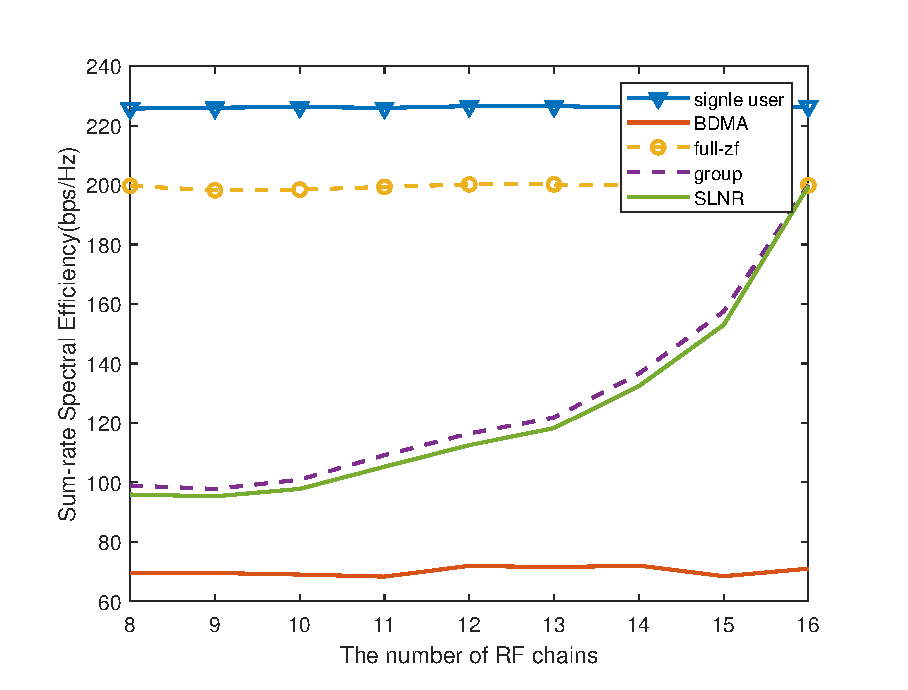
\includegraphics[width=3.8in,height=3.2in]{Figure/NRFChains.eps}
		\caption{Different number of RF chains.}\label{fig:RFchains}
	\end{center}
\end{figure}
In the Fig.~\ref{fig:RFchains}, we can see that the sum-rate capacity will increase as more RF chains added.


\begin{figure}[ht]
	\begin{center}
		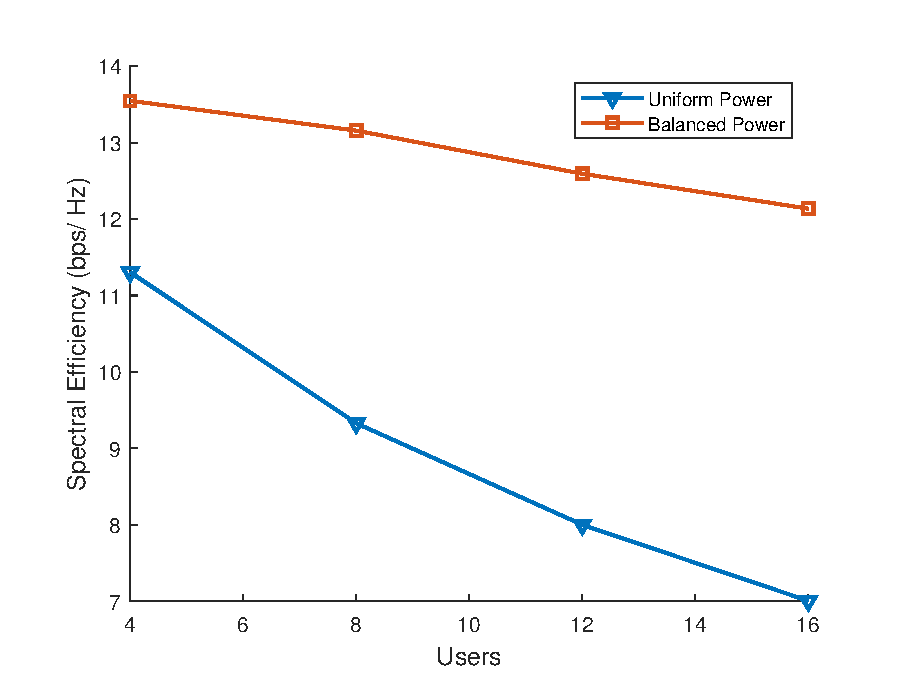
\includegraphics[width=3.8in,height=3in]{Figure/powerBalanced.eps}
		\caption{Power allocation.}\label{fig:CDF}
	\end{center}
\end{figure}


Finally, we study the multiuser gain provided by opportunistic scheduling. By varying the number of active users, we investigate the sum-rate capacity improvement. Fig.~\ref{fig:MultiuserGain} shows that PAPRA-OHBF can significantly benefit from the increase of active users as the number of active users grows from $6$ to $20$. However, the benefit of having more active users diminishes as the number of active users increases beyond $30$. In contrast, the non-opportunistic analog beamforming is not capable of reaping multiuser gains. As a result, the curve labelled ``Analog Beamforming" does not change much with the number of active users.	

\bibliography{BDMAref}
\bibliographystyle{IEEEtran}


% references section

\end{document}


